\documentclass{article}
\usepackage[T1]{fontenc}
\usepackage[utf8]{inputenc}
\usepackage{mathptmx}
\usepackage[margin=0.75in,columnsep=0.3in]{geometry}
\usepackage{multicol}
\usepackage{graphicx}
\usepackage{booktabs}
\usepackage{amsmath}
\usepackage[hidelinks]{hyperref}

\setlength{\columnsep}{0.3in}

\title{\Large\bfseries Forecasting EV Registration Growth in New York State:\\A Controlled Comparison of Five Methods Under a Trend Reversal}
\author{Akhilesh Vangala\\ \small Center for Data Science, New York University \\ \small sv3129@nyu.edu}
\date{}

\begin{document}
\twocolumn[
\begin{@twocolumnfalse}
\maketitle
\begin{abstract}
\noindent Utilization data for individual EV fast-charging stations is commercially
licensed and not publicly available, so this project asks a narrower question: using
only public New York State DMV and charging-infrastructure data, can county-level EV
registration growth be forecast reliably enough to be useful for site selection. We
build a reproducible pipeline over 210{,}774 registered electric vehicles and 5{,}501
public charging stations, then compare five forecasting methods -- a naive last-year
baseline, an OLS linear trend, Holt linear exponential smoothing, Random Forest, and
LightGBM -- on a 2024--2025 holdout. Every method more sophisticated than the naive
baseline loses to it, and the size of the loss (naive RMSE 481; OLS 686; Random Forest
1{,}175; LightGBM 1{,}526; Holt 2{,}246) tracks almost exactly how strongly each
method's inductive bias assumes the trend continues. The reason is a real regime
change: statewide registrations grew every year from 2018 through 2023, then declined
in both 2024 and 2025. We decompose each method's error into bias and variance
components, show LightGBM's forecast is driven almost entirely by one- and two-year
lag features, and use the resulting zip-level charging-station data to flag 129 New
York City zip codes with 50 or more registered EVs and zero DC fast chargers.
\end{abstract}
\end{@twocolumnfalse}
]

\section{Introduction}
Electric vehicle charging site selection depends on a forecast of future demand, and
the data that would forecast it most directly -- per-station session counts, dwell
time, uptime -- is sold by vendors such as Paren and Atlas Public Policy rather than
published. This project builds the closest available substitute from public data:
New York State DMV vehicle registration snapshots and a state-maintained directory of
public charging stations. Rather than assume a single model is the right one to trust,
we hold everything constant except the forecasting method -- same counties, same
holdout years, same features where applicable -- and compare five methods that make
progressively stronger assumptions about trend continuation.

Our questions are simple: which method wins on a real holdout, is the winner an
artifact of an easy holdout window, and what does the losing methods' failure actually
look like once decomposed. The answer to the second question turns out to be the most
useful finding in the project.

\section{Data}
Two live New York State open-data sources and one federal geography file are pulled
and cached by \texttt{src/ingest.py}:

\begin{itemize}
\setlength\itemsep{0.2em}
\item \textbf{NY DMV Vehicle Registrations} (data.ny.gov, \texttt{w4pv-hbkt}): filtered
to \texttt{fuel\_type=ELECTRIC} and \texttt{record\_type=VEH}, giving 210{,}774
electric vehicles across 62 counties and 1{,}907 zip codes, model years 2011--2026.
\item \textbf{NY EV Charging Stations} (data.ny.gov, \texttt{7rrd-248n}): 5{,}501
public charging locations with Level 1, Level 2, and DC fast port counts per zip.
\item \textbf{Census Gazetteer ZCTA file}: land area per zip code, used for density
rather than population, which is not available without an API key.
\end{itemize}

Model year is used as a proxy for adoption timing: it is not a perfect stand-in for the
calendar year a vehicle was first registered, but it is the only year field the DMV
snapshot exposes, and it is stated as a limitation throughout rather than treated as
exact. County-year counts are built by grouping registrations by county and model
year, reindexing every county across the full 2011--2025 year range so that a county
with zero new registrations in a given year is recorded as zero rather than missing.
Two lag features (one and two years back) and a year index are derived from this
series for the tree-based and naive methods.

\section{Methods}
All five methods are trained on model years 2011--2023 and evaluated on a strictly
held-out 2024--2025 window per county, with the final partial year (2026) excluded
from both training and evaluation entirely.

\textbf{Naive} predicts next year's count as equal to last year's -- no trend
assumption at all. \textbf{OLS trend} fits one ordinary least squares line per county
across the full training window. \textbf{Holt linear} (Holt, 1957) fits an
exponentially-smoothed level and trend per county and extrapolates the trend forward
with no bound. \textbf{Random Forest} (Breiman, 2001) and \textbf{LightGBM} (Ke et al.,
2017) are both trained on four features -- year index, a county indicator, and the
two lag features -- pooled across all counties, with 300 trees (depth 6) and 200
boosting rounds (depth 4, learning rate 0.05) respectively.

For each method we report RMSE, MAE, MAPE, and a bias-variance decomposition of the
holdout error: bias is the mean signed error, and the variance component is defined so
that the two recompose exactly to RMSE:
\begin{equation}
\text{variance component} = \sqrt{\max(\text{RMSE}^2 - \text{bias}^2,\ 0)}
\end{equation}

\section{Results}

\subsection{Main comparison}
Table~\ref{tab:main} and Figure~\ref{fig:comparison} report holdout results. The naive
baseline wins outright: RMSE 481 versus 686 for OLS trend, 1{,}175 for Random Forest,
1{,}526 for LightGBM, and 2{,}246 for Holt linear.

\begin{table}[h]
\centering
\small
\caption{Holdout results, model years 2024--2025.}
\label{tab:main}
\begin{tabular}{lrrr}
\toprule
Model & RMSE & MAE & Bias \\
\midrule
Naive (last year) & 481 & 162 & +84 \\
OLS trend & 686 & 264 & -236 \\
Random Forest & 1{,}175 & 601 & +514 \\
LightGBM & 1{,}526 & 730 & +669 \\
Holt linear & 2{,}246 & 759 & +757 \\
\bottomrule
\end{tabular}
\end{table}

\begin{figure}[h]
\centering
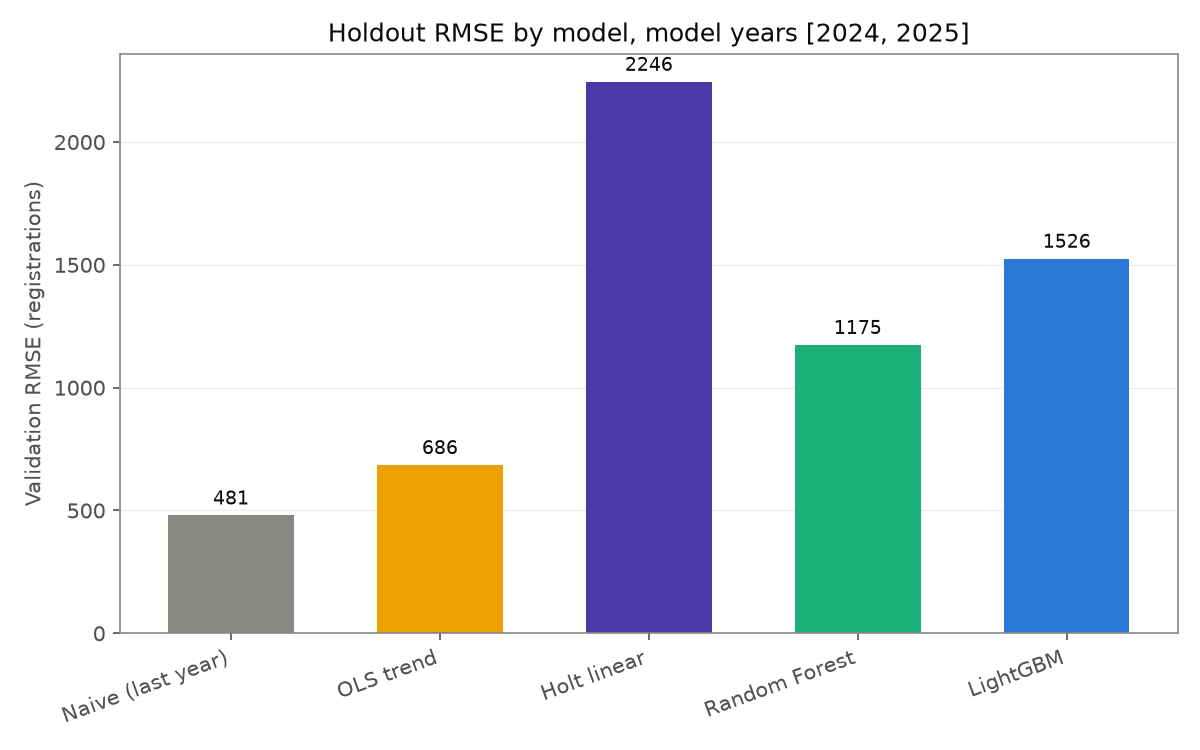
\includegraphics[width=\linewidth]{../figures/model_comparison.png}
\caption{Holdout RMSE by model. The ordering tracks how strongly each method
extrapolates trend, not general model quality.}
\label{fig:comparison}
\end{figure}

\subsection{Why the naive baseline wins}
Figure~\ref{fig:growth} shows why: statewide new registrations rose from 11{,}795
(2021) to a peak of 48{,}411 (2023), then fell to 44{,}396 (2024) and 38{,}046 (2025) --
two consecutive years of decline after five years of acceleration. Every method except
naive was trained on a window that ends in uninterrupted growth, and each extrapolates
that growth by an amount proportional to how directly its structure encodes a trend.
Holt linear extrapolates an explicit, unbounded trend term and has both the worst RMSE
(2{,}246) and the largest bias (+757). Random Forest and LightGBM split on lag
features, which bounds their extrapolation to values seen in training, producing
smaller but still large positive bias (+514 and +669). OLS is the only
non-naive method with negative bias (-236): a single line fit across the entire
2011--2023 window is pulled down by the early, near-flat years enough to partially
offset the late acceleration it is also trying to fit.

\begin{figure}[h]
\centering
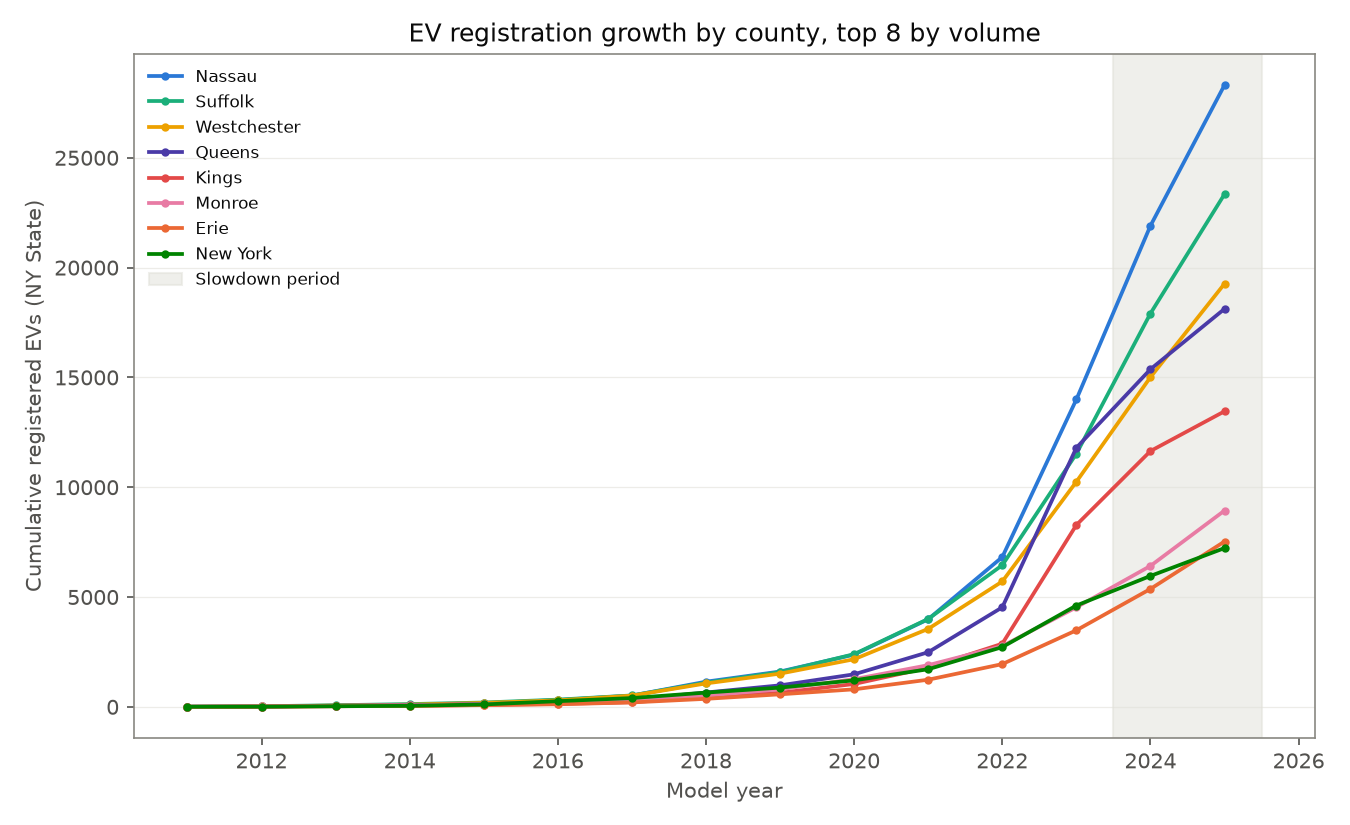
\includegraphics[width=\linewidth]{../figures/county_growth_curves.png}
\caption{Cumulative registrations for the top 8 counties by volume. All show the same
flattening after 2023 (shaded region).}
\label{fig:growth}
\end{figure}

\begin{figure}[h]
\centering
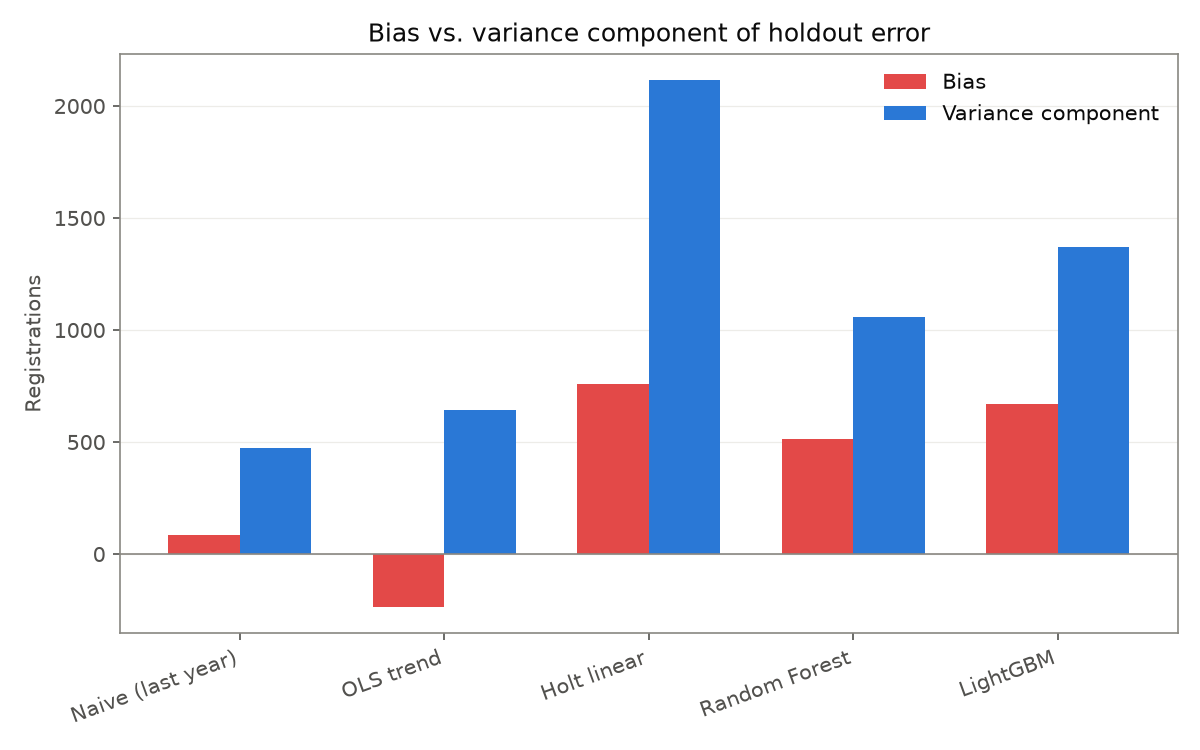
\includegraphics[width=\linewidth]{../figures/bias_variance.png}
\caption{Bias and variance components of holdout RMSE. Every non-naive method is
bias-dominated in the same direction: over-prediction.}
\label{fig:biasvar}
\end{figure}

\subsection{Where LightGBM fails and what drives it}
Figure~\ref{fig:worst} breaks LightGBM's holdout error down by county. New York
(Manhattan) county has the single worst error (RMSE 4{,}716) and it is almost entirely
bias (4{,}716) rather than variance (40) -- on a county with only two holdout points,
the model was confidently and consistently wrong in one direction, which is as much a
small-sample warning as a modeling one. Orange and Rockland counties split their error
more evenly between bias and variance, suggesting a noisier underlying trend rather
than a single systematic miss.

Figure~\ref{fig:importance} shows why LightGBM behaves this way: by total gain, the
one- and two-year lag features dominate the model, with year index and the county
indicator contributing much less. LightGBM is, in effect, a flexible way of looking at
recent history, which is exactly why it is hurt by the same regime change that hurts
Holt: recent history stopped being a reliable guide to what came next.

\begin{figure}[h]
\centering
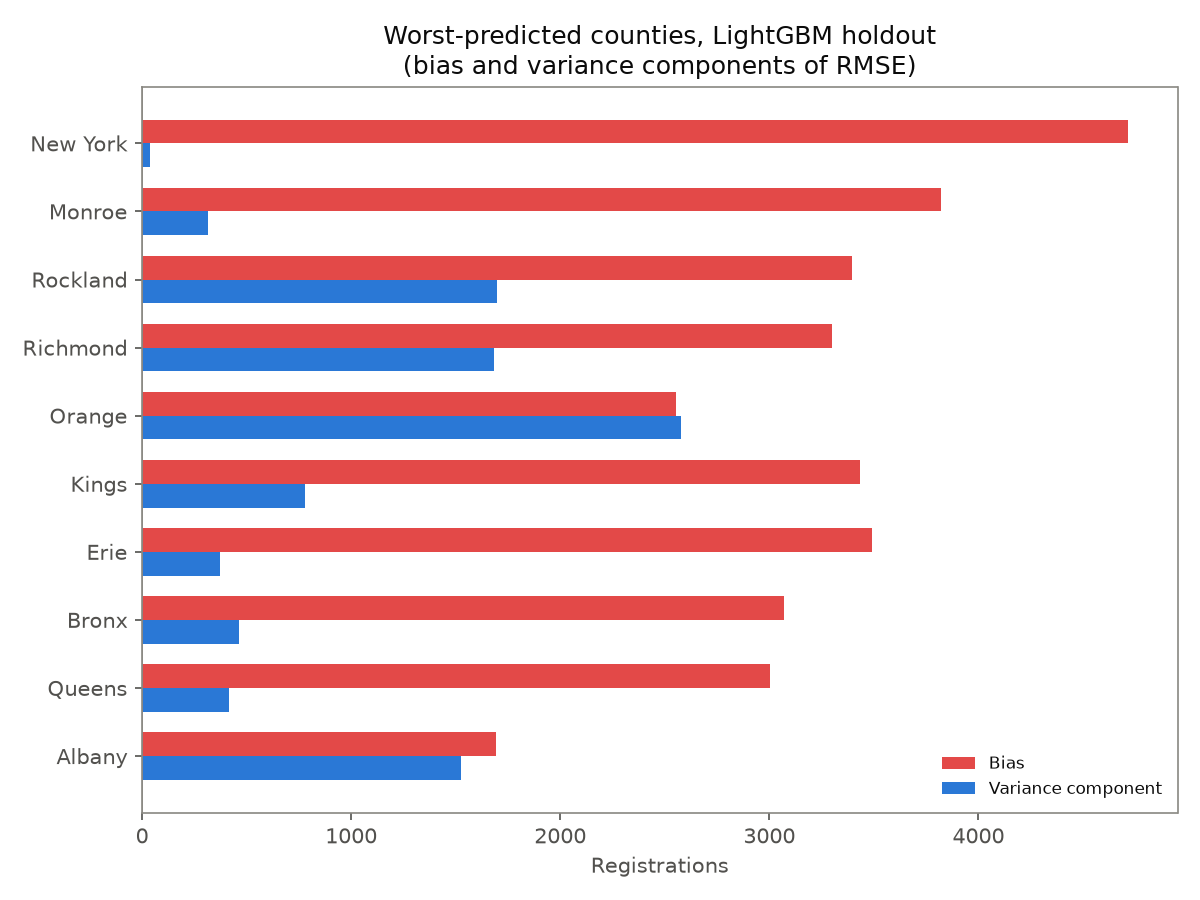
\includegraphics[width=\linewidth]{../figures/worst_counties.png}
\caption{Bias and variance components of LightGBM holdout error, worst 10 counties.}
\label{fig:worst}
\end{figure}

\begin{figure}[h]
\centering
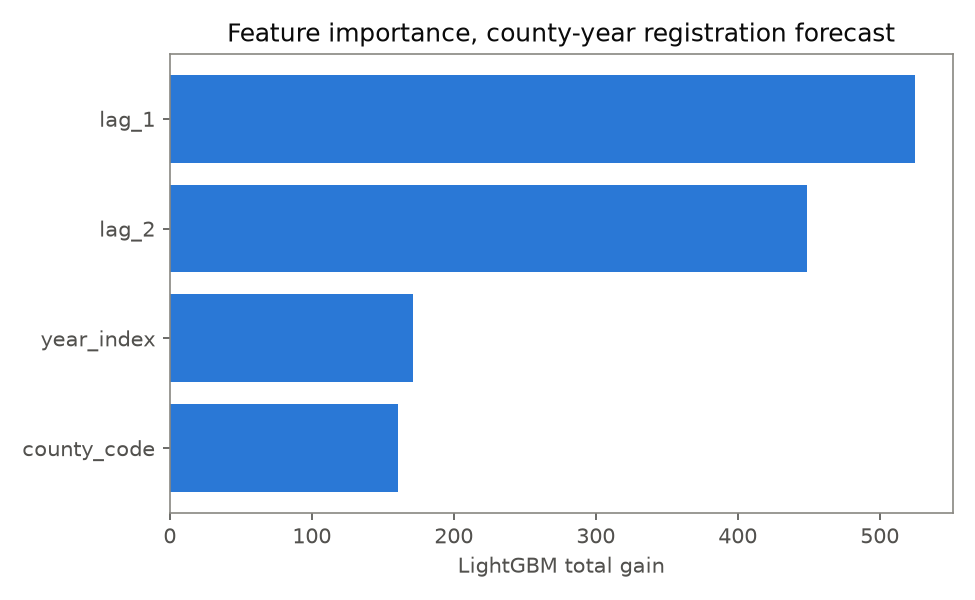
\includegraphics[width=0.85\linewidth]{../figures/feature_importance.png}
\caption{LightGBM feature importance by total gain. Lag features dominate.}
\label{fig:importance}
\end{figure}

\subsection{Application: where NYC charging supply lags registered demand}
Independent of the forecasting comparison, the same cleaned registration and station
data can answer a simpler question: where is the gap between registered EVs and
existing charging supply largest today. Figure~\ref{fig:gap} ranks New York City zip
codes with at least 20 registered EVs by registered EVs per public charging port.
Restricting to zip codes with 50 or more registered EVs, 129 zip codes across the five
NYC counties have zero DC fast charging ports at all.

\begin{figure}[h]
\centering
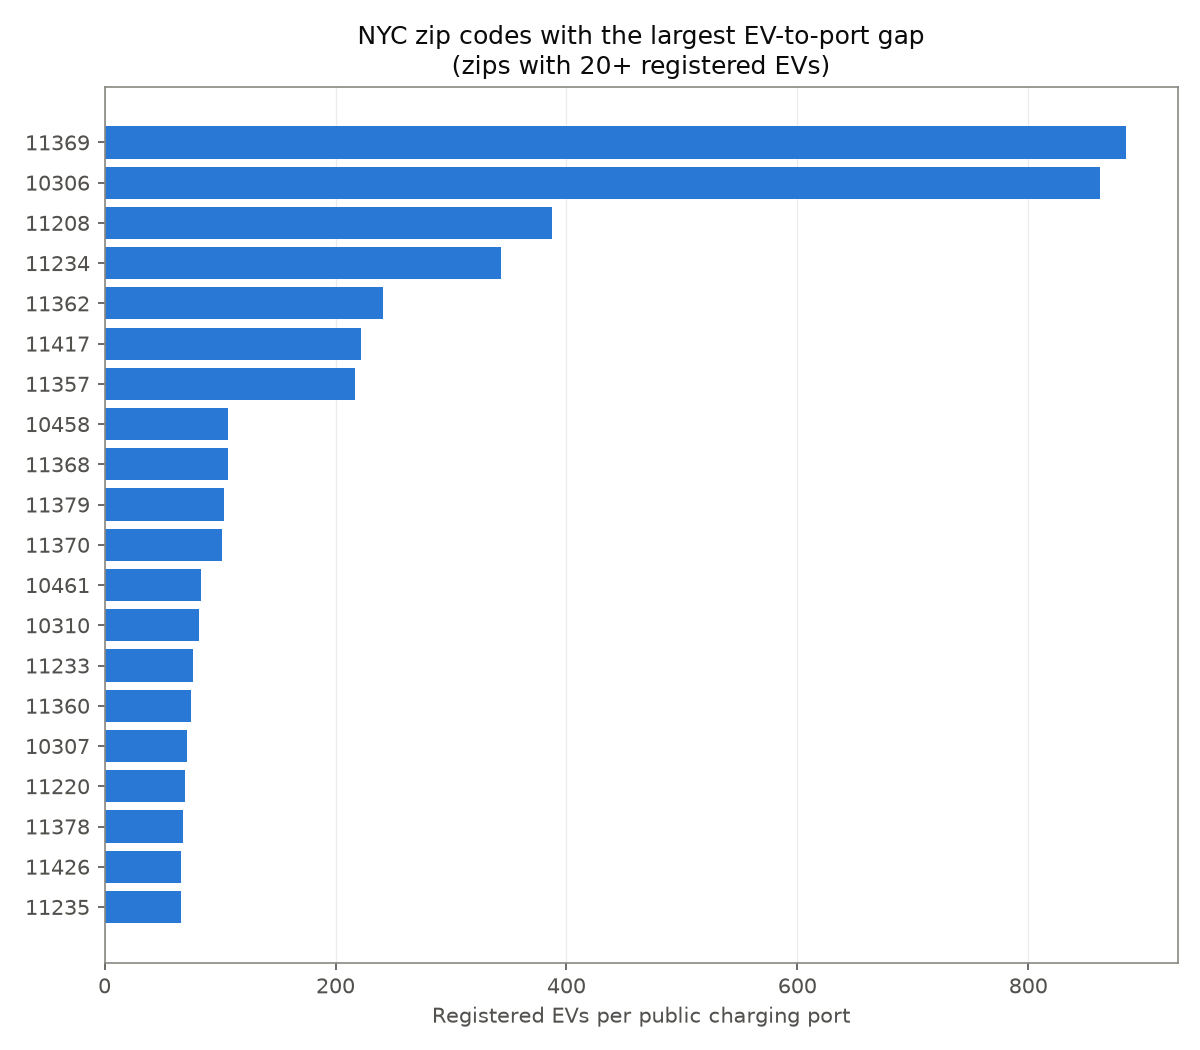
\includegraphics[width=\linewidth]{../figures/nyc_demand_gap.png}
\caption{NYC zip codes with the largest ratio of registered EVs to existing charging
ports.}
\label{fig:gap}
\end{figure}

\section{Discussion}
The headline result is not that naive forecasting is a good strategy in general --
it is that a holdout period which happens to break the training trend will make every
trend-aware method look worse than a method with no opinion about trend at all, and
that this is worth reporting plainly rather than picking a friendlier holdout window.
A production forecasting system for this problem would need either an explicit
regime-change detector or wide enough uncertainty bands to survive being wrong about
one, and neither is something a single point-accuracy metric on a lucky holdout window
would reveal.

\section{Conclusion}
Across five forecasting methods evaluated identically on the same New York State EV
registration data, holdout accuracy ordering tracked each method's willingness to
extrapolate a training-period trend, and the least sophisticated method won because
the trend it would have extrapolated had already reversed. The bias-variance
decomposition shows this clearly: every method beyond naive is bias-dominated in the
same direction, and the size of that bias scales with how directly the method encodes
recent trend. Separately, the same pipeline surfaces 129 New York City zip codes with
real registered EV demand and no DC fast charging access today, which does not depend
on any forecast being correct.

\section*{Code and Data}
All code, tests, and result files are available at {\small
\href{https://github.com/Akhilesh-Vangala/ev-charging-demand-forecasting}{github.com/Akhilesh-Vangala/\allowbreak ev-charging-demand-forecasting}}.

\begin{thebibliography}{9}
\bibitem{breiman} L. Breiman, ``Random forests,'' \textit{Machine Learning}, vol. 45,
no. 1, pp. 5--32, 2001.
\bibitem{lightgbm} G. Ke et al., ``LightGBM: A highly efficient gradient boosting
decision tree,'' \textit{Advances in Neural Information Processing Systems}, vol. 30,
2017.
\bibitem{holt} C. C. Holt, ``Forecasting seasonals and trends by exponentially
weighted moving averages,'' \textit{ONR Memorandum}, no. 52, 1957 (reprinted
\textit{International Journal of Forecasting}, 2004).
\bibitem{ny-dmv} New York State Department of Motor Vehicles, ``Vehicle, Snowmobile,
and Boat Registrations,'' data.ny.gov, resource w4pv-hbkt, 2026.
\bibitem{ny-stations} New York State, ``Electric Vehicle Charging Stations in New
York,'' data.ny.gov, resource 7rrd-248n, 2026.
\bibitem{paren} Paren, ``State of the Industry: DC Fast Charging,'' paren.app, 2026.
\end{thebibliography}

\end{document}
